\documentclass[conference, a4paper,10pt,twocolumn]{IEEEtran}

\usepackage{graphics} % for pdf, bitmapped graphics files
\usepackage{epsfig} % for postscript graphics files
\usepackage{mathptmx} % assumes new font selection scheme installed
\usepackage{times} % assumes new font selection scheme installed
\usepackage{amsmath} % assumes amsmath package installed
\usepackage{amssymb}  % assumes amsmath package installed
\usepackage{psfrag}
\usepackage{subfigure}
\usepackage{cite}
\usepackage{amsthm}
\usepackage{flushend}

% correct bad hyphenation here
\hyphenation{op-tical net-works semi-conduc-tor IEEEtran}

\begin{document}

\title{A simple approach to WSN monitoring}

% avoiding spaces at the end of the author lines is not a problem with
% conference papers because we don't use \thanks or \IEEEmembership

% use only for invited papers
%\specialpapernotice{(Invited Paper) }

% make the title area
\maketitle
%\footnote{}
\begin{abstract}

We report on a wireless sensor network (WSN) architecture including a 
local sensor network, a gateway and uplinks to Internet. We also report 
on experiences from its use in data acquisition and monitoring applications.
The architecture is based on basic rather than advanced WSN mechanisms 
to avoid complexity, prioritize robustness and quick deployment and to 
facilitate operation, management and maintenance.
The protocol architecture involves a unified information structure for 
sensor data from mote to central repository and power saving light 
weight protocols in the local sensor network part.
The hardware core of the architecture is a wireless sensor network node
(mote) based on a micro-controller integrating an ADC and radio
transceiver, on-board sensors and means to connect external sensors. The 
current Contiki-based firmware revision implements broadcasting and 
relaying. When connected to a gateway via a serial connection (USB), the 
mote acts as a sink node forwarding all reports received to the gateway 
controlled by a daemon using the unified and flexible tagged  data format.
The gateway maintains alternative uplinks and TCP streams to facilitate
transmission of data to a central repository via Internet.
The power supply for the sensor nodes is based on ultra capacitors and 
solar panels.
End user interfaces include raw data access, data plots and
mobile apps. Our report also includes performance measurements and
experiences from field tests.

\end{abstract}

\begin{IEEEkeywords} 
Internet of Things, IoT, 6LowPAN, Wireless sensor networks, WSN, Contiki, RIME
 \end{IEEEkeywords}


% no keywords

% For peer review papers, you can put extra information on the cover
% page as needed:
% \begin{center} \bfseries EDICS Category: 3-BBND \end{center}
%
% for peerreview papers, inserts a page break and creates the second title.
% Will be ignored for other modes.
% \IEEEpeerreviewmaketitle

\section{Introduction}
\label{sec:intro}
 
The motivation behind this work on wireless sensor networks comes from 
our participation in a number projects involving data acquisition and 
monitoring of important environment data at off-grid locations lacking 
most sorts of infrastructure, especially network connectivity and power 
supply, and having poor supply chains~\cite{UBIQUI}.

As a consequence, our focus has been on robustness, power consumption 
and simplicity in installation, operation, management and maintenance.

Wireless sensor networks have been subject to research for almost two 
decades and to standardization for at least one. Together with 
applications and wired infrastructure, they are an important part of 
Internet of Things when the protocols used are compatible with the 
Internet protocol architecture. Various link level protocols have been 
explored. Until recently, the IEEE 802.15.4~\cite{802154}  link level 
standard [ieee802.15.4] has been dominating.

On the network level, the IETF 6lowpan group has recently concluded its 
effort to define a standard for transmitting IPv6 packets over 802.15.4 
links ~\cite{6LOWPAN}. A new IETF group has been chartered with a wider scope 
[6lo].

On the routing side, there is a broad spectrum of solutions assuming 
more or less complex network topologies.  A basic network topology, that 
we have adopted in the work reported in this paper, uses one hop 
broadcasting of all motes, except a sink mote connected to a gateway 
with uplinks to Internet. In the wireless sensor network, between the 
motes, we use a less power-consuming addressing scheme than ipv6 
discussed further below. All motes, except the sink mote, spend most of 
their time in a power-saving mode. They just wake up, do their 
measurement, report and go back to deep sleep. 

A simple mechanism to extend the network over one hop has been added.
This requires the extending or relaying node to have radio in listening 
mode as the network is unsynchronized. We have left the more complex 
solutions based on relaying mesh network topologies and power-saving 
radio duty cycling for further studies.

On the application level, there is a need for a flexible data structure 
for all sorts of sensor data to be transported between the motes and the 
gateway and further on via uplinks to users. We have chosen to use plain 
text in the reports and to include tags also in plain text defining the 
data in the report, both between motes, in the file storage and over the 
uplinks. The reports also include a time stamp and configurable 
identifiers. 

The protocol used over the uplink is plain TCP thus enabling apps like 
nc, telnet, standard web-browser to directly monitor the raw data.
Gateway can be entended to support other uplink protcols.

The hardware and software system architectures developed for 
implementation of wireless sensor networks include a wide spectrum of 
embedded system hardware and operating systems for for structuring 
microcontroller firmware.
On the hardware side, we chose to use the ATMEL Atmega128RF component 
integrating a microcontrollerm a 10bit ADC with 8 channels and an ieee 
802.15.4 transceiver~\cite{ATMEGA}.
On the software side, we evaluated two of the more commonly used, 
Contiki~\cite{CONTIKI} and TinyOS~\cite{tinyos}. We found Contiki having 
a smaller memory footprint and fitted our C, Linux and Github platforms 
better. Contiki includes RIME, a small and simple adressing scheme for 
WSN communication that we chose instead of ipv6. There is a new 
interesting candidate, mbed, announced by the ARM consortium 
~\cite{mbed}, but not yet available enough for our purposes in the 
context of this paper.


In section ~\ref{sec:needs} , we discuss a more detailed needs and requirement analysis for the use cases
In section ~\ref{sec:architecture}, we present the overall architecture
In section ~\ref{sec:implementation}, we present details about current implementation  
In section ~\ref{sec:experince}, we present an installation and actual usage
Finally, in section ~\ref{sec:conclusion}, we present our conclusions and suggestions for further studies.
\section{Needs and requirements}
%%\label{sec:Needs and requirements}
\label{sec:needs}


There is a need for low-power devices to keep installations small and cost-effective also for 
flexible power design. In many installations the temperatures are high. This decreasing 
battery lifetime and adding the need maintenance and cost.

Our low power hardware can be placed in deep sleep between measurements and transmissions.  The key 
components in our design include  Contiki-OS~\cite{CONTIKI} running on Atmel ATMega128RF~\cite{ATMEGA} 
integrating an MCU, an IEEE 802.15.4-compatible~\cite{802154} radio transceiver and an 8-channel 10-bit 
AD-converter. This component has been used to design a WSN mote with some additional components such 
as an EUI64 address chip, voltage converters, a temperature sensor, etc. When in deep sleep, the MCU 
itself consumes ~1$\mu$A and the entire mote ~10-15$\mu$A. When transmitting, the mote consumes 
~20mA. At 3V, this means ~60mW. 

The performance and coverage of the IEEE 802.15.4 depending on a lot of factors. Antenna, output
power and of course transmission disturbances but with the used PCB-antenna 100m line of sight and 
beyond is possible. The long range can have negative impact in high density networks but for simple 
and small and medium scale installations this can an advantage.


\section{Architecture}
\label{sec:architecture}
 

\subsection{Network topology}

IoT devices and sensors has three major mapping to the Internet. The 
or node cen exposed via

\begin{itemize}

\item Native IP address. Ether IPv4 or IPv6. 6LowPAN constitutes IPv6


\item Via a IP gateway. Gateway can of course have IPv4 or IPv6. Protocol
can be any native IP protocols or IP protocols specially designed 
for constrained applications like CoAP or MQTT etc. The gateway 
translates between two standardized internet protocol stacks. 


\item  Via IP gateway but in this case a non IP address are used on
the nodes examles Contki's RIME, Zigbee . The gateway translates 
between two protocol stacks. 

\end{itemize}

I our implementations we're using RIME on the WSN-nodes. I should
be pointed out that our TDF data tagging does not require this.

RIME is a lightweight protocol with a very low overhead. Header is 
16 bit's. The current implementation uses a RIME broadcast network
the 16 bit source address is composed by a globally unique EUI64 
address chip on located every node this to get an unique RIME-
address. 



\section{Implementation}
\label{sec:implementation}



\subsection{Report and sink nodes}

A report or broadcast node sends the sensor data from local 
node, temp, RH etc, or any more other connected instruments 
or sensors.

This report is sent periodically via a configurable report
interval. The radio is only active during the sending the 
report which is a very short time.

Figure ~\ref{fig:bcast} illustrates this.

As a result the whole Micro Controller Unit (MCU) be in deep 
sleep and be woken up by a timer and to send it's data.

The sink node or receiving node is listening and collecting
the broadcast reports. This node is connected to the IP gateway
using USB over the TTL-UART.  There can be several sink nodes
in a network. This sink node can itself have sensors and to
report the gateway.

\subsection{Power needs}

As the network is unsynchronized the sink node must be listing
all time. This gives a higher current consumption on the sink node. 
In our case about 18mA. The new version of the AtMega128RF chip 
claims to have reduced consumption in listening mode. ~\cite{ATMEGA}

While the sink node needs some power all reporting nodes 
can spend almost it's time in the deepest sleep. Just to woken 
up by a timer read the desired sensors and go to the deepest 
sleep again. 

The memory oscilloscope traces in figure~\ref{fig:bcast} 
and figure~\ref{fig:bcast-detail} show the current consumption 
of the MCU when the radio transmits one Contiki RIME~\cite{RIME} 
broadcast packet per second. 
We see short spikes at 17mA. In this experiment, the MCU sleep 
mode was changed from ``Idle'' to ``Power save'' after four seconds.

The authors has worked on a new and innovative power design 
for sensor nodes. The design is based on the novel advances 
in supercapacitor technology. In the mentioned work ~\cite{LICCAP}  
a reporting has shown to run 6 weeks reporting every minute
on a single Lithium-Ion-Capacitor. The time to fully charge 
a capacitor is in minutes and can be done by a solar panel.

Of course it's the total power consumption thats effects 
the operational time. 

\begin{figure}
\centering
    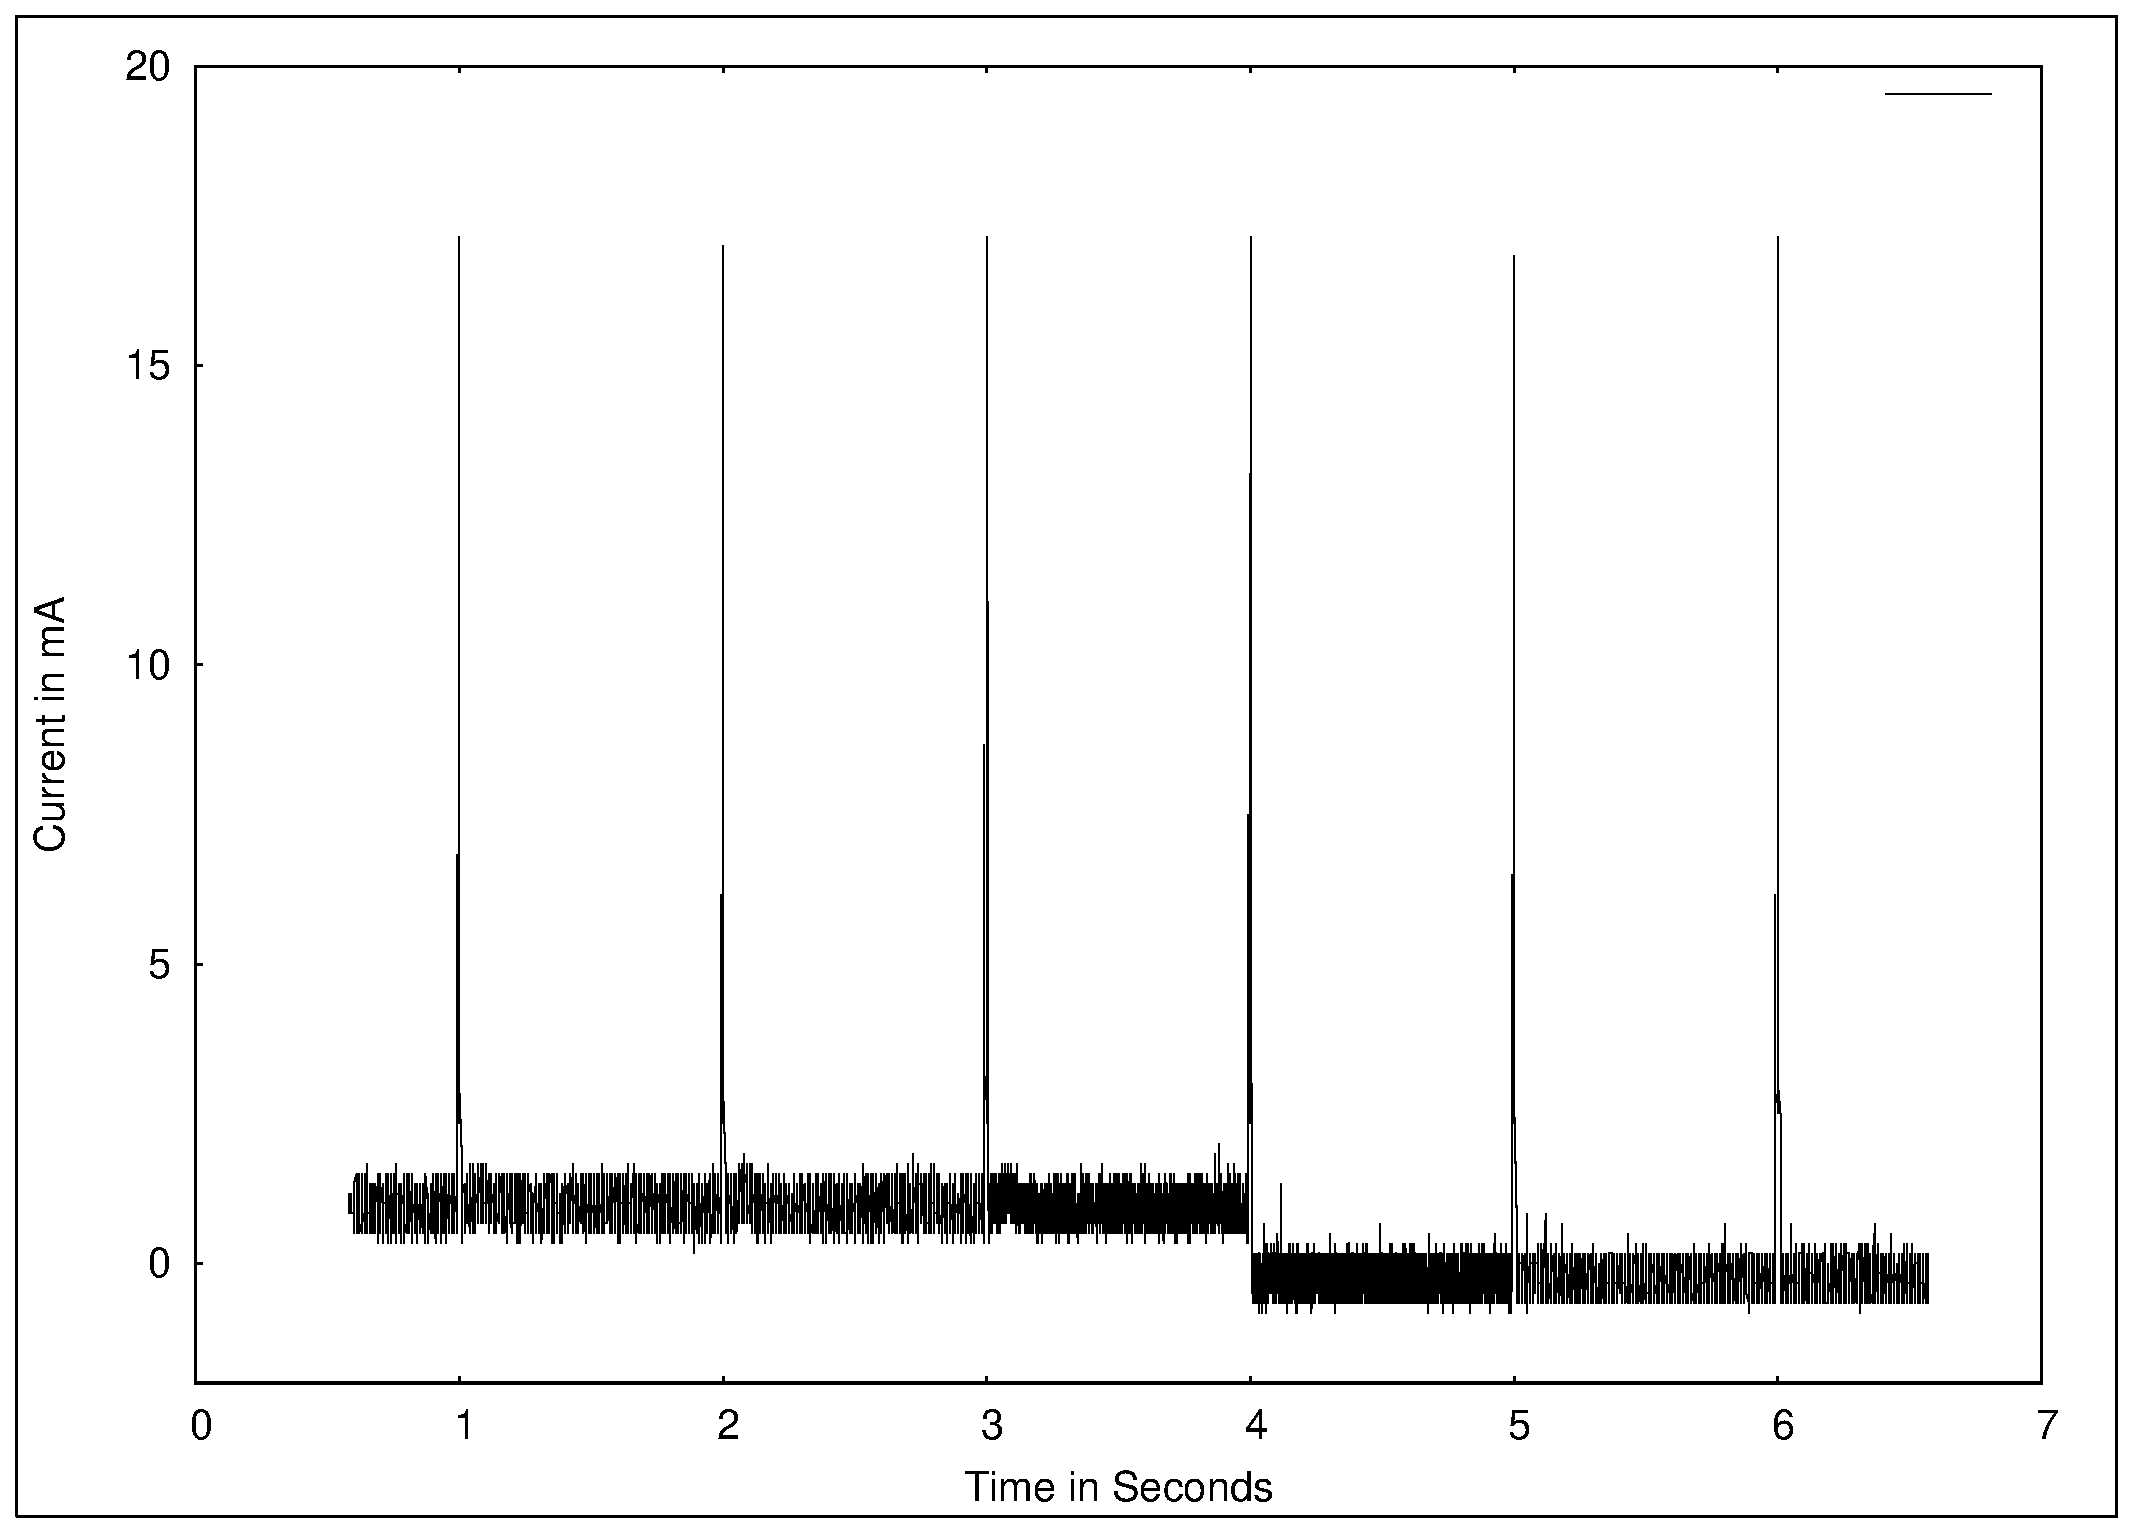
\includegraphics[width=3.4in]{bcast.eps}
    \caption{Periodic broadcast of Contiki RIME packets with 1 sec interval with ATMega128rfa1 ieee 802.15.4 radio output at 3dBm using MCU Sleep mode “IDLE” during the first 4 seconds and MCU sleep mode “PWR-SAVE” thereafter.}
    \label{fig:bcast}
\end{figure}


\begin{figure}
\centering
    \includegraphics[width=3.4in]{bcast-detail.eps}
    \caption{Close-up of one of the transmissions with MCU in Sleep mode in PWR-SAVE}
    \label{fig:bcast-detail}
\end{figure}



\subsection{Data format}
Here
Stateless vs stateful monitoring can be discussed. 


\subsection{Gateway}
The gateway gives IP connectivity to the WSN network and all the 
reachable sensor nodes. In our case we're using TCP for communication 
with the gateway.  sensd ~\cite{sensd} is the used a gateway implemented
as a unix style daemon. Typically sensd has a sink node connected over 
serial/USB. Sensd reads all data report from the sink node. 

When a TCP client is connected to sensd all the WSN received reports  
are distributed th the client(s) using TCP. There can be many TCP 
clients connected to the gateway at the same. All shaing the same data.
Sensd acts like a hub or rendez-vous point for data sharing of the 
WSN network.

As data is encoded in ASCII simple TCP utilities like nc, netcat, 
telnet or web browsers can be used to monitor the data. Also there 
are specialized apps for telephones. 

\subsection{Gateway and proxy}
In some installations the WSN network is behind a NAT. 
This impliess that the gateway can not be reached from 
the Internet. To solve this problem functionality was 
add sensd to forward data to remote server.
If the server is globally reachable this works becomes an
proxy function. TCP clients can connect the same way to 
the proxy server to receive the sensors reports initiated 
behind the NAT.

Several WSN network can be merged inro a single proxy server. 
This opens for interesting possibilities how subset of nodes 
can selected etc.

\subsection{Plot and utilities}
Here

\subsection{App support}
Here we discuss Read Sensors App  ~\cite{read-sensors}

\subsection{Data repository and storage}
Here

\subsection{Multihop networking: Contolled relay}

\section{Experiences and Installations}
\label{sec:experince}

\section{Conclusions and further work}
\label{sec:conclusion}

We see research directions to follow:

\begin{itemize}
\item Access control of nodes and data. 

\item Merge of data flows 

\item If possible an more compact data representation and alinment to CoAP, MQTT etc

\end{itemize}

Issues for further study include: 

\begin{itemize}
\item Scalability of network
\item Practical and robust implementation
\item Security
\item Data integrity and security

\end{itemize} 

The authors are currently involved in field studies including these issues

\begin{thebibliography}{1}

\bibitem{UBIQUI} Amos Nungu, Robert Olsson, Bj\"{o}rn Pehrson. \emph{Implementation of Inclusive Ubiquitous Access}. 
Journal of Wireless Personal Communication, 2012

\bibitem{6LOWPAN}  Z. Shelby and C. Bormann, \emph{6LoWPAN: The Wireless Embedded Internet}
Wiley, Ed.Wiley, November 2009

\bibitem{802154}  \emph{IEEE 802.15.4}. 
[Online]. Available: http://www.ieee802.org/15/pub/TG4.html. [Accessed: 21-February-2012]

\bibitem{CONTIKI}  \emph{The Contiki Os.}. 
[Online]. Available: http://www.contiki-os.org/. [Accessed: 29-February-2012].

\bibitem{RIME} Adam Dunkels. \emph{Rime - a lightweight layered communication stack for sensor networks}.   In Proceedings of the European Conference on Wireless Sensor Networks (EWSN), Poster/Demo session, Delft, The Netherlands, January 2007.

\bibitem{ATMEGA} Atmel Corporation. \emph{ATmega128RFA1}. 
[Online]. Available: http://www.atmel.com/devices/ATMEGA128RFA1.aspx. [Accessed: 21-February-2012].

\bibitem{ATMEGAR2} Atmel Corporation. \emph{ATmega128RFR2}. 
[Online]. Available: http://www.atmel.com/devices/atmega128rfr2.aspx?tab=documents [Accessed: 01-July-2015].


\bibitem{RSS2} Radio Sensors mote. \emph{RSS2}. 
[Online]. Available: http://radio-sensors.com/ [Accessed: 16-June-2015]

\bibitem{LICCAP} Robert Olsson, Bj\"{o}rn Pehrson. \emph{Powering devices using ultra-capacitor batteries}
[Publishing Pending]

\bibitem{UBIQUISTATUS} [Amos Nungu, Robert Olsson, Bj\"{o}rn Pehrson, Jiawei Kang, Daniel Kifetew, Alisher Rustamov]. \emph{Inclusive Ubiquitous Access - A Status Report}. 
Africom, Younde, Nov 2012

\bibitem{SBN} SBN. \emph{IL2213 WSN-Projects Fall 2011.}. 
[Online]. Available: http://www.tslab.ssvl.kth.se/csd/files/wsn/index.html. [Accessed: 21-February-2012].

\bibitem{sensd}  \emph{sensd gateway}. 
[Online]. Available: https://github.com/herjulf/sensd [Accessed: 16-June-2015]

\bibitem{read-sensors}  \emph{Read-Sensors Android app}. 
[Online]. Available: https://github.com/herjulf/Read-Sensors [Accessed: 16-June-2015]


\bibitem{ODROID} \emph{Odroid U3 and C1}
[Online]. Available: http://www.hardkernel.com [Accessed 5-April-2015]
\end{thebibliography}
\end{document}

